In this section, we will present the execution time of the basic ROMC
functionalities. Apart from performing the inference accurately, one
of the notable advantages of ROMC is its efficiency. In terms of
performance, ROMC holds two key advantages.

Firstly, all its subparts are parallelisable; optimising the objective
functions, constructing the bounding boxes, fitting the local
surrogate models, sampling and evaluating the posterior can be
executed in a fully-parallel fashion. Therefore, the speed-up can be
extended as much as the computational resources allow. Specifically,
at the CPU level, the parallelisation can be incorporate all available
cores. A similar design can be utilised in the case of having a
cluster of PCs available. Parallelising the process at the GPU level
is not that trivial, since the parallel tasks are more complicated
than simple floating-point operations. Our current implementation
supports parallelisation at the training part: at solving the
optimisation problems and at constructing the bounding
boxes.\footnote{The design of our code permits adding this feature at
  all the aforementioned tasks at a future update.}. In subsection
\ref{subsubsec:parallel}, we will demonstrate the speed-up achieved
through parallelisation.

The second significant advantage concerns the execution of the
training and the inference phase in distinct timeslots. Therefore, one
can consume a lot of training time and resources but ask for
accelerated inference. The use of a lightweight surrogate model around
the optimal point exploits this essential characteristic; it trades
some additional computational burden at the training phase, for
exercising faster inference later. In figures \ref{fig:exec_solve},
\ref{fig:exec_regions}, \ref{fig:exec_posterior},
\ref{fig:exec_sample} we can only observe this advantage. The
example measured in these figures is the simple 1D example, used in
the previous chapter. We observe that fitting local surrogate models
slows down the training phase (estimating the regions) by a factor of
$1.5$, but provides a speed-up of $15$ at the inference phase i.e.\
approximating unnormalised posterior. This outcome would be even more
potent in larger models, where running the simulator is even more
expensive.


\begin{figure}[ht]
    \begin{center}
      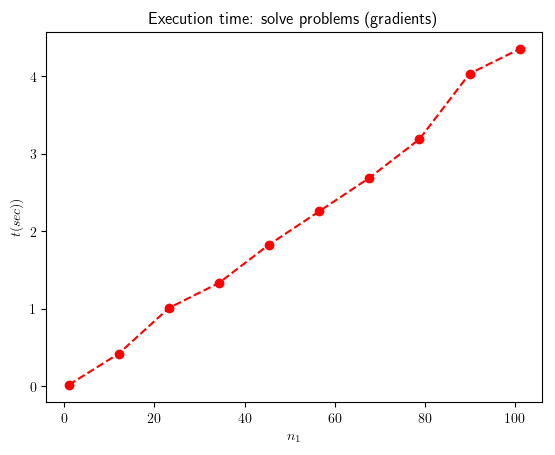
\includegraphics[width=0.48\textwidth]{./Thesis/images/chapter4/exec_solve_grad.png}
      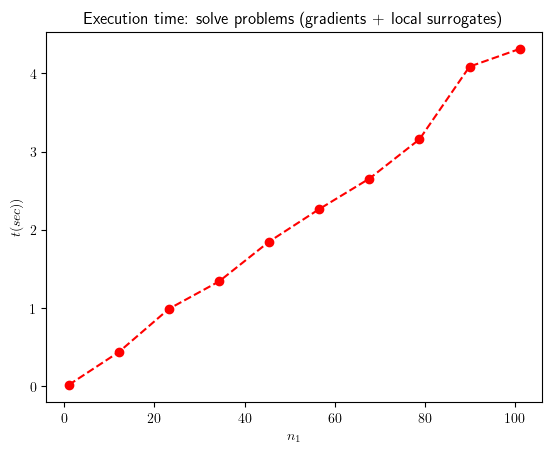
\includegraphics[width=0.48\textwidth]{./Thesis/images/chapter4/exec_solve_grad_fit.png}\\
      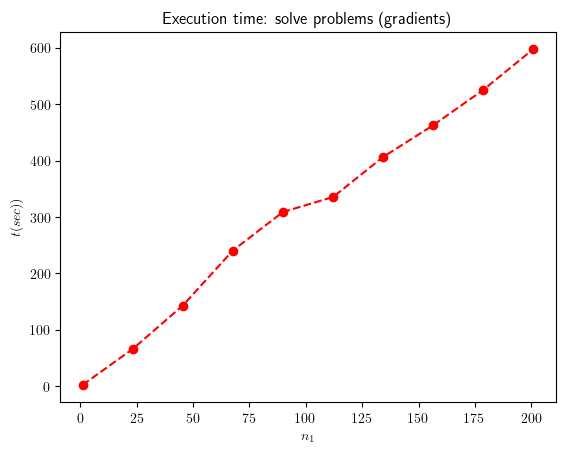
\includegraphics[width=0.48\textwidth]{./Thesis/images/chapter4/exec_solve_bo.png}
      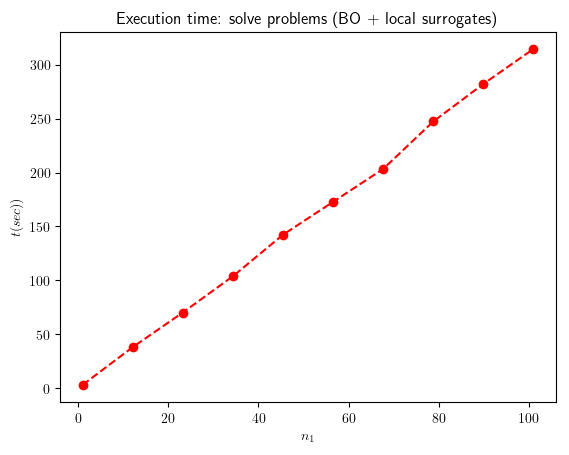
\includegraphics[width=0.48\textwidth]{./Thesis/images/chapter4/exec_solve_bo_fit.png}          \end{center}
    \caption[Execution time for solving the optimisation problems.]{Execution time for defining and solving the optimisation
      problems. We observe an increase by a factor of $75$ when switching
      to Bayesian optimisation scheme.}
  \label{fig:exec_solve}
\end{figure}


\begin{figure}[ht]
    \begin{center}
      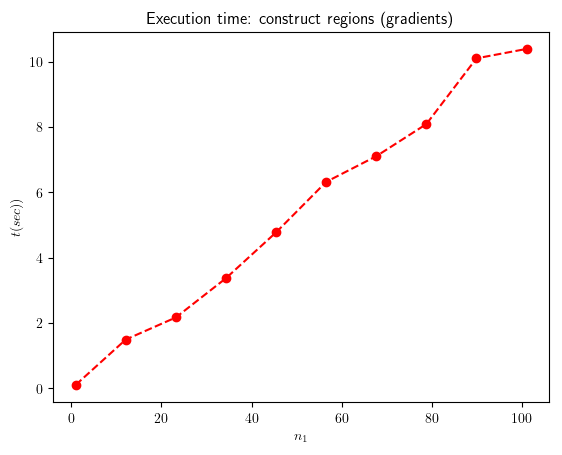
\includegraphics[width=0.48\textwidth]{./Thesis/images/chapter4/exec_regions_grad.png}
      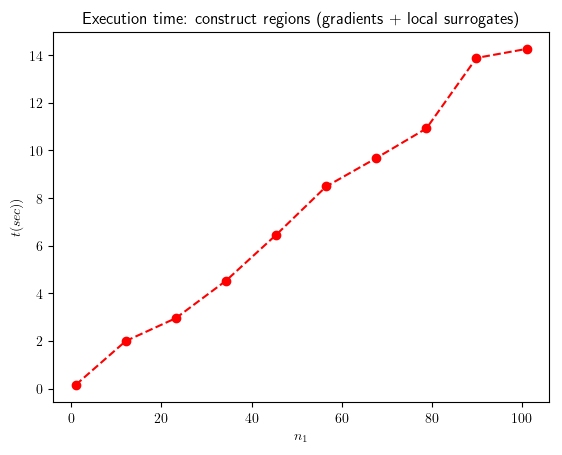
\includegraphics[width=0.48\textwidth]{./Thesis/images/chapter4/exec_regions_grad_fit.png}\\
      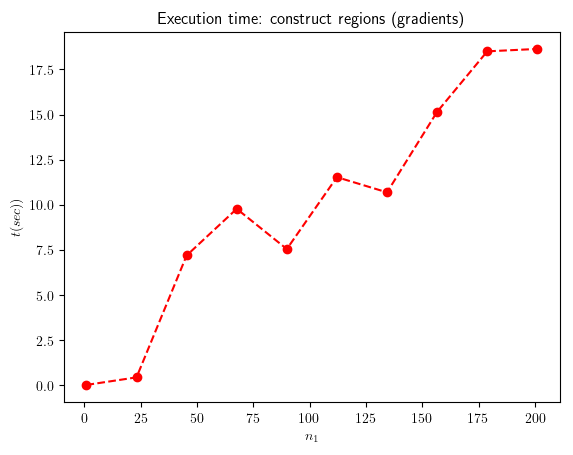
\includegraphics[width=0.48\textwidth]{./Thesis/images/chapter4/exec_regions_bo.png}
      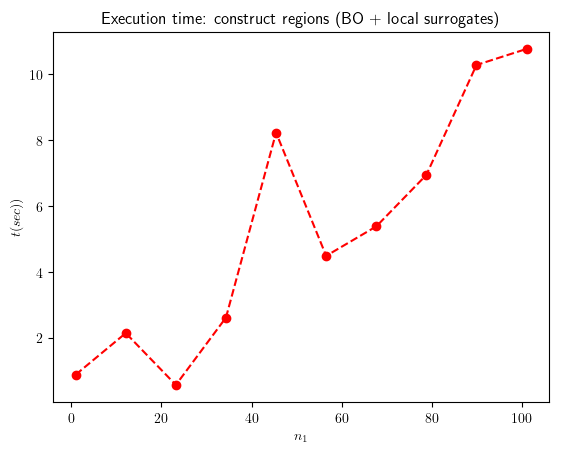
\includegraphics[width=0.48\textwidth]{./Thesis/images/chapter4/exec_regions_bo_fit.png}
    \end{center}
    \caption[Execution time for constructing the n-dimensional bounding box regions.]{Execution time for constructing the n-dimensional
      bounding box region and, optionally, fitting the local surrogate
      models. We observe that fitting the surrogate models incurs a
      small increase by a factor of $1.5$.}
  \label{fig:exec_regions}
\end{figure}


\begin{figure}[ht]
    \begin{center}
      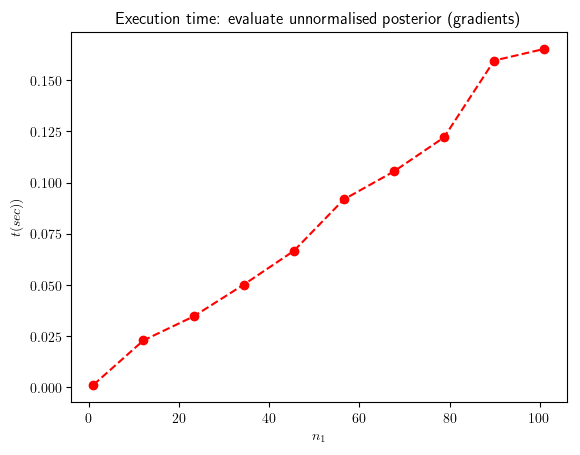
\includegraphics[width=0.48\textwidth]{./Thesis/images/chapter4/exec_posterior_grad.png}
      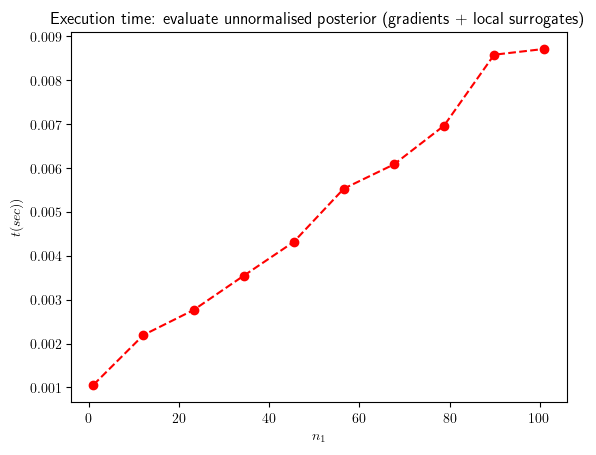
\includegraphics[width=0.48\textwidth]{./Thesis/images/chapter4/exec_posterior_grad_fit.png}\\
      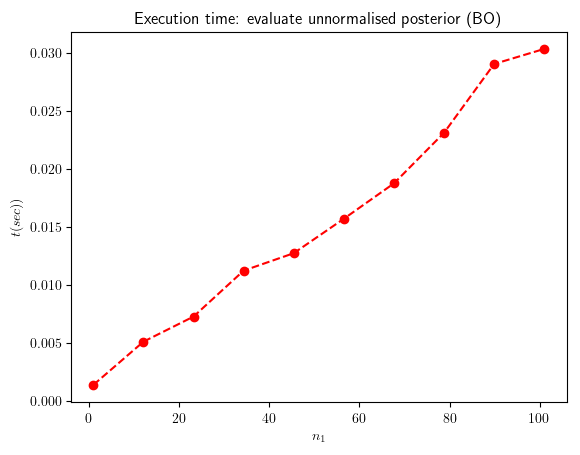
\includegraphics[width=0.48\textwidth]{./Thesis/images/chapter4/exec_posterior_bo.png}
      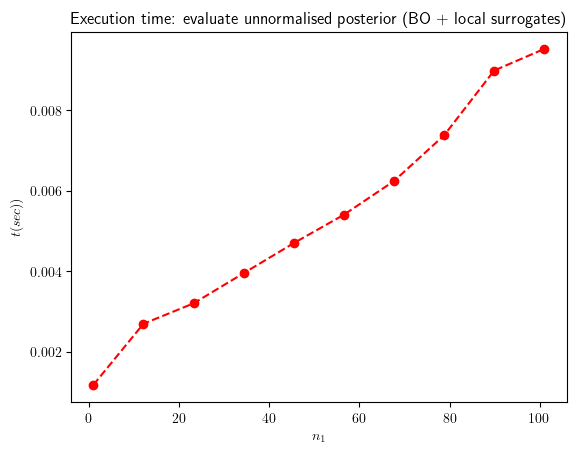
\includegraphics[width=0.48\textwidth]{./Thesis/images/chapter4/exec_posterior_bo_fit.png}
    \end{center}
    \caption[Execution time for evaluation the unnormalised posterior.]{Execution time for evaluating the unnormalised posterior
      approximation. We observe that there is a major speed-up in the
      models with fitted local surrogate models, by about a factor $15$.}
  \label{fig:exec_posterior}
\end{figure}


\begin{figure}[ht]
    \begin{center}
      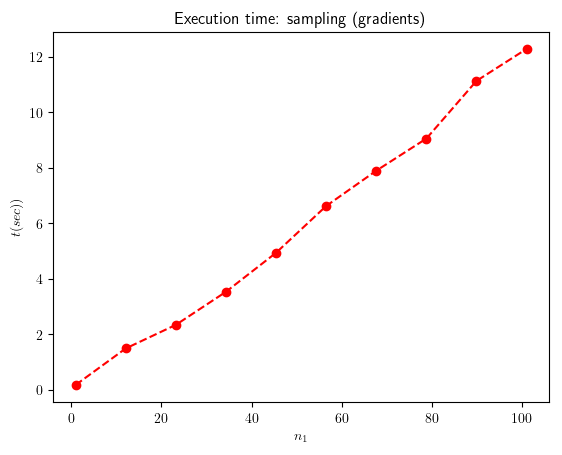
\includegraphics[width=0.48\textwidth]{./Thesis/images/chapter4/exec_sample_grad.png}
      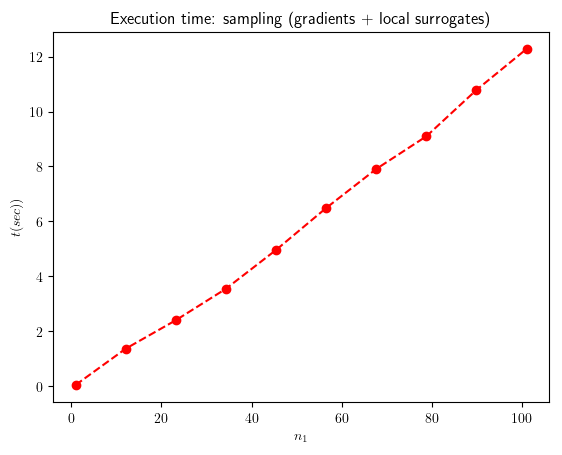
\includegraphics[width=0.48\textwidth]{./Thesis/images/chapter4/exec_sample_grad_fit.png}\\
      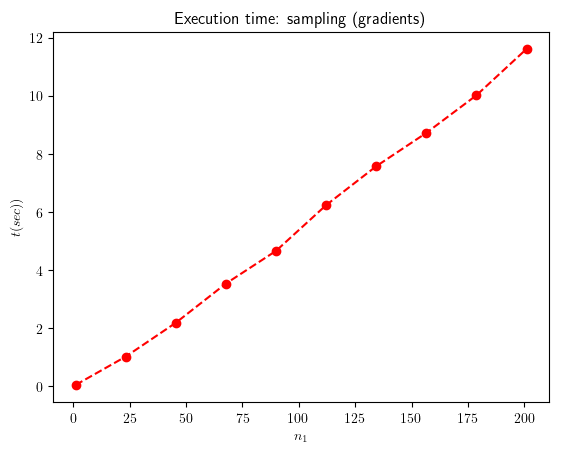
\includegraphics[width=0.48\textwidth]{./Thesis/images/chapter4/exec_sample_bo.png}
      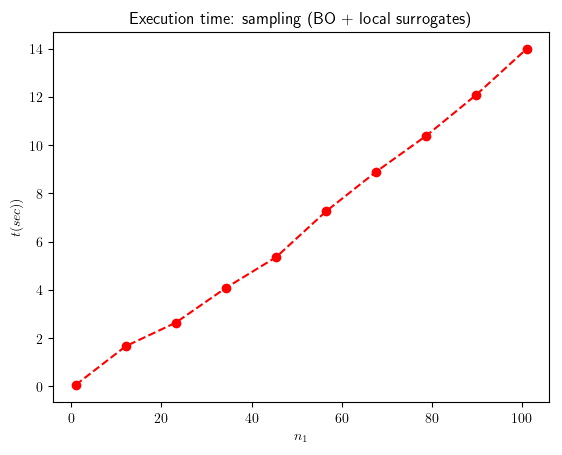
\includegraphics[width=0.48\textwidth]{./Thesis/images/chapter4/exec_sample_bo_fit.png}
    \end{center}
    \caption[Execution time for sampling from the approximate posterior.]{Execution time for sampling from the approximate
      posterior. We observe a small speed-up when the local surrogate
      models are fitted, by about a factor $1.5$.}
  \label{fig:exec_sample}
\end{figure}


\subsubsection{The effect of parallelisation} \label{subsubsec:parallel}

Solving the optimisation problems and estimating the bounding boxes
can be done in a fully parallel way, since the tasks are completely
independent. In figure \label{fig:exec_parallel}, we measure the
execution times with and without parallelisation at the simple 1D
example. In the experiments we use a cpu with 8 cores, therefore the
theoretical (maximum) speed-up can reach a factor of 8. Normally the
observed speed-up is a little bit lower due to the overhead of
setting-up the parallel processes. Our experiments confirm our general
expectation; in both the sequential and the parallel case, the
execution time increases linearly with the number $n_1$, though with a
different slope coefficient. At solving the optimisation problems, the
slope coefficient is almost 6 times smaller, whereas at constructing
the bounding boxes 2.5 times smaller, with small deviations.

\begin{figure}[ht]
    \begin{center}
      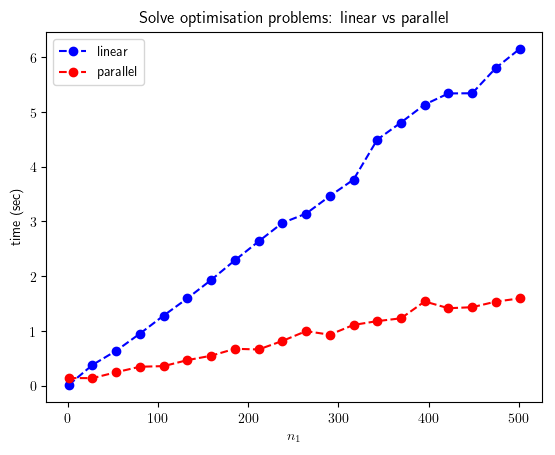
\includegraphics[width=0.48\textwidth]{./Thesis/images/chapter4/solve_problems_parallel.png}
      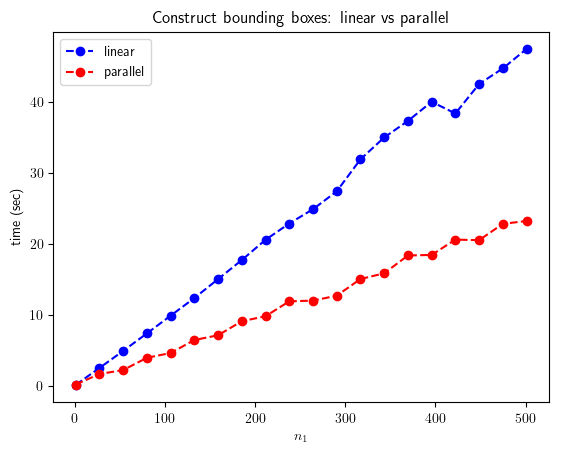
\includegraphics[width=0.48\textwidth]{./Thesis/images/chapter4/estimate_regions_parallel.png}
    \end{center}
    \caption[Execution time exploiting parallelisation.]{Execution
      time exploiting parallelisation. At the left figure, we measure
      the execution time for solving the optimisation problems. At the
      right figure, we measure the execution time for constructing the
      bounding boxes.}
  \label{fig:exec_parallel}
\end{figure}
